% Manuscript skeleton for the 11/25 OpenReview submission.
% Build: pdflatex main && bibtex main && pdflatex main && pdflatex main (no LaTeX on the lab server; use Overleaf).
% Every number is traceable to a results file: see README.md. "TODO" marks text still to write or verify.
\documentclass[10pt]{article}
\usepackage[margin=1in]{geometry}
\usepackage{amsmath,amssymb}
\usepackage{booktabs}
\usepackage{graphicx}
\usepackage{multirow}
\usepackage[numbers]{natbib}
\usepackage{hyperref}
\usepackage{xcolor}
\newcommand{\todo}[1]{\textcolor{red}{[TODO: #1]}}

\title{Learning Individual Walking-Style Preferences for Crowd Navigation\\from a Few Pairwise Queries}
\author{Anonymous}
\date{}

\begin{document}
\maketitle

% 11/18 abstract, updated with the DPO and candidate-generator results (11/20) and the information-gain / robustness runs (11/23).
\begin{abstract}
People differ in how they want a robot to move through a crowd: some prefer it to yield early, others to keep pace;
some want it to pass behind them, others in front. Existing crowd-navigation policies optimize a fixed notion of social
compliance and cannot adapt to such individual preferences. We present a framework that identifies a user's walking-style
preference from a handful of pairwise (A/B) queries and uses it to select the robot's path at test time. A VQ-VAE trained on
human pedestrian trajectories provides a codebook of walking behaviours that generates style-diverse, human-like candidate paths.
Unsafe candidates are filtered out, and each remaining candidate is described by interpretable style features: passing side,
passing in front or behind, yielding, detour width, and human-likeness. A Bayesian Bradley--Terry model over these features is
updated after each answer, and queries are chosen by the expected utility of the best option (EUBO). On held-out situations from
Grand Central and ETH/UCY with simulated users, five queries reduce the normalized simple regret from 0.45--0.47 (human-data prior)
to 0.09--0.12, outperforming random queries in all four settings and a DPO-trained estimator on the same budget and matching an
information-gain query; the advantage over random queries persists when simulated users answer noisily or have nonlinear preferences. On shared
Grand Central scenes, codebook candidates leave 0.11 regret after five queries against 0.35 for candidates from a flow-matching
crowd-navigation generator, whose narrower candidate set bounds what any preference can achieve. In a closed-loop replay,
following the learned preference keeps the user's step regret low without raising the collision rate.
\end{abstract}

\section{Introduction}
\label{sec:intro}

\begin{figure*}[t]
  \centering
  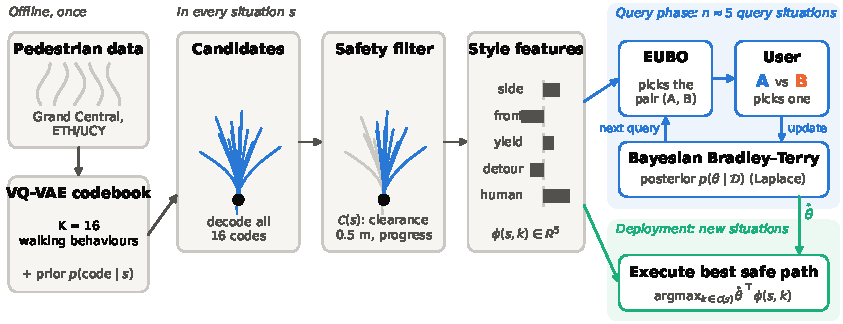
\includegraphics[width=\linewidth]{figures/fig_architecture.pdf}
  \caption{Framework. Offline, a VQ-VAE learns a codebook of $K=16$ walking behaviours and a prior network from pedestrian
  trajectories. In every situation the codebook is decoded into candidate paths, unsafe ones are removed, and each safe candidate is
  described by five style features. In a few query situations EUBO picks a pair of safe candidates, the user answers which they prefer,
  and a Bayesian Bradley--Terry posterior over the preference is updated. In new situations, without further questions, the robot
  executes the safe candidate that is best under the posterior mean $\hat\theta$. Fig.~\ref{fig:overview} shows the steps on a real
  situation. Generated by \texttt{utils/figure\_architecture.py}.}
  \label{fig:architecture}
\end{figure*}

Robots increasingly share sidewalks, stations and shopping streets with people, and how such a robot moves through a crowd matters to
the person it serves -- the user who sends a delivery robot, rides in a wheelchair or walks alongside a guide robot. ``Socially compliant''
navigation, however, is not a single behaviour. Facing an oncoming pedestrian, one user wants the robot to slow down and let them pass,
another wants it to keep pace; one prefers it to pass behind people, another in front; one tolerates a wide detour around a group, another
wants the shortest safe path. People themselves differ in how close they pass others and how readily they give way
\citep{hall1966hidden}, so a single notion of good crowd behaviour leaves many users
dissatisfied.

Crowd-navigation methods nonetheless optimize one fixed objective. Model-based planners encode hand-tuned social costs, reinforcement-learning
policies maximize a designed reward, and imitation or generative planners reproduce the average pedestrian of their training data
\citep{helbing1995social,vandenberg2011reciprocal,chen2019crowd,kretzschmar2016socially,mavrogiannis2023core}. Adapting any of them to an individual requires retuning or
retraining. Preference-based learning offers a direct route: instead of specifying a reward, the user compares two behaviours and the robot
infers what they want~\citep{christiano2017deep,sadigh2017active}. In robotics, however, each comparison costs the user time and attention,
so a preference must be identified from a handful of answers, and the trajectories being compared must be meaningful to a person: safe,
plausible, and different in ways the user cares about.

Our key idea is to separate \emph{what} the robot can do from \emph{which} of those behaviours a particular user wants (Fig.~\ref{fig:architecture}).
For the first, we learn a discrete codebook of human walking behaviours with a VQ-VAE~\citep{vandenoord2017neural} trained on pedestrian
trajectories. Decoding the codebook in a given situation yields a small set of candidate paths that are human-like by construction and
differ in style -- passing left or right, ahead or behind, slowing down or keeping pace -- and a safety filter removes the ones that come too
close to anyone. For the second, we describe each safe candidate by five interpretable style features and model the user's preference as a
linear utility over them, learned with a Bayesian Bradley--Terry model~\citep{bradley1952rank} from A/B answers. Because the robot only
executes one path per situation after querying, the relevant objective is simple regret, and we choose each question by the expected utility
of the best option (EUBO)~\citep{astudillo2023qeubo}, which is one-step Bayes-optimal for it.

The data prior alone does not capture individual preferences: on held-out situations from Grand Central and ETH/UCY, always taking the most
human-like safe path leaves a normalized simple regret of 0.45--0.47 for simulated users, close to a random safe path (0.49). Five EUBO
queries reduce it to 0.09--0.12, with lower regret than random questions in all four settings and than an active-query baseline in three,
and as low as an information-gain query; the advantage over random questions holds for noisy, inconsistent and nonlinear simulated users.
The comparison with Direct Preference Optimization~\citep{rafailov2023direct}, the estimator behind much of current preference fine-tuning,
shows where the gain comes from: given the same questions, DPO and the Bradley--Terry posterior perform alike, but DPO has no posterior with
which to choose its questions. The candidate set matters as well: on shared Grand Central scenes, the candidates of a flow-matching
crowd-navigation planner~\citep{singha2026crowdfm} cover a much narrower range of behaviours than the codebook, which bounds what any learned preference
can achieve (union regret 0.35 vs 0.11 after five queries). Finally, in a closed-loop replay, following the learned preference keeps the
user's step regret at 0.10--0.14 without a significant change in collision rate.

\paragraph{Contributions.}
\begin{itemize}
  \item A walking-behaviour codebook learned with a VQ-VAE from pedestrian trajectories, which turns a situation into a small set of
        diverse, human-like candidate paths that a safety filter can check (Sec.~\ref{sec:candidates}).
  \item A linear preference over five interpretable style features, learned with a Bayesian Bradley--Terry model from A/B answers,
        with questions chosen by EUBO to minimize simple regret (Sec.~\ref{sec:preference}).
  \item A simple-regret evaluation protocol on held-out situations (Sec.~\ref{sec:regret}) and experiments on Grand Central and
        ETH/UCY that compare query selection (including information gain and users outside the model), a DPO estimator, a flow-matching candidate generator, and closed-loop execution
        (Sec.~\ref{sec:experiments}).
\end{itemize}

\section{Related Work}
\label{sec:related}

\paragraph{Crowd navigation.}
% Model-based (social force, ORCA), learned (RL, imitation), generative planners (diffusion / flow matching).
% Point: they optimize one fixed notion of social compliance.
\todo{write; cite social force, ORCA, CADRL/SARL-type RL, and the flow-matching planner used as our baseline generator}

\paragraph{Learning from pairwise preferences.}
Pairwise comparisons are commonly modelled with the Bradley--Terry model~\citep{bradley1952rank}. Preference-based reward learning
was scaled up with deep networks by \citet{christiano2017deep} and became the basis of RLHF for language models~\citep{ouyang2022training}.
Direct Preference Optimization~\citep{rafailov2023direct} removes the separate reward model and fits the policy to the preference pairs
directly, with a KL anchor to a reference policy; we use it as an estimator baseline.
\todo{2--3 sentences on how this differs from our setting: few answers per user, choice among a small safe set}

\paragraph{Active preference queries in robotics.}
\citet{sadigh2017active} select trajectory comparisons that maximize information about a linear reward.
EUBO~\citep{astudillo2023qeubo} asks the pair maximizing the expected utility of the better option and is one-step Bayes-optimal for
simple regret; we adopt it because our objective is the one path executed after querying.
\todo{cite the active-query (version-space) baseline (UserAlign) once the reference is confirmed}

\paragraph{Discrete behaviour representations.}
VQ-VAEs~\citep{vandenoord2017neural} learn a discrete codebook; \todo{cite trajectory/motion codebook works (motion primitives, VQ for trajectory prediction)}.

\section{Method}
\label{sec:method}

% Fig. 1 (pipeline) \todo{draw: situation -> codebook candidates -> safety filter -> style features -> A/B queries (EUBO) -> theta -> executed path}

\subsection{Problem setting}
In a situation $s$ the robot knows its own state (speed, two past positions), its destination and the positions and velocities of
nearby people. A user has a preference over how the robot walks, which we model as a linear utility over style features.
The user answers a small number of A/B questions in a few query situations; the robot must then choose its path in new situations
the user was never asked about.

\subsection{Walking-behaviour codebook}
\label{sec:candidates}
A VQ-VAE~\citep{vandenoord2017neural} with $K=16$ codes is trained on pedestrian futures expressed in the heading frame as deviations
from constant velocity (6 points every 0.8\,s, 4.8\,s). Decoding every code from the robot's current speed gives $K$ candidate paths.
A prior network $p(\text{code} \mid s)$, trained on the same data with the destination and a summary of nearby people as input,
scores how typical each candidate is for a person in that situation.
\todo{training details: data split by person, epochs, prior inputs; GC: 12,159 test conflict situations; ETH/UCY: 590}

\paragraph{Safety filter.}
People are extrapolated at constant velocity; a candidate is safe if its minimum distance to everyone is at least $c=0.5$\,m and its
progress towards the destination is at least $\rho=0.5$ times the best candidate's. The preference only chooses among safe candidates:
\begin{equation}
  \mathcal{C}(s) = \bigl\{ k \;:\; d_{\min}(s,k) \ge c,\; \mathrm{prog}(s,k) \ge \rho \max_{k'} \mathrm{prog}(s,k') \bigr\}.
\end{equation}

\subsection{Style features}
Each safe candidate is described by $\phi(s,k) \in \mathbb{R}^5$, none of which has an a-priori right sign:
\emph{side} ($\tanh$ of the lateral offset from the conflict person at closest approach),
\emph{front} (crossing ahead of or behind them), \emph{yield} (mean speed relative to the current speed),
\emph{detour} (largest deviation from the straight line to the destination) and \emph{human} ($\log p(\text{code}\mid s)$).
Features are standardized over the safe candidates of the query situations.

\subsection{Preference learning and query selection}
\label{sec:preference}
The user's utility is $u(s,k) = \theta^\top \phi(s,k)$. Answers follow the Bradley--Terry model~\citep{bradley1952rank}
$P(i \succ j \mid \theta) = \sigma(\theta^\top(\phi_i - \phi_j))$ with prior $\theta \sim \mathcal{N}(0, I)$; the posterior is
approximated by a Laplace approximation (Newton's method for the MAP, inverse Hessian as covariance).
Each query asks the pair maximizing the expected utility of the best option~\citep{astudillo2023qeubo},
\begin{equation}
  (i,j) = \operatorname*{arg\,max}_{i \ne j} \; \mathbb{E}_{\theta \sim p(\theta \mid \mathcal{D})}\bigl[\max\{u_i, u_j\}\bigr],
\end{equation}
estimated with 512 posterior samples. At test time the robot executes
$\hat k_n(s) = \arg\max_{k \in \mathcal{C}(s)} \hat\theta_n^\top \phi(s,k)$ with $\hat\theta_n$ the posterior mean after $n$ answers.

% Formal regret definition (11/18 feedback item 4). Setting, safe set and executed path are defined in Sec. 3.
\subsection{Evaluation: simple regret}
\label{sec:regret}

\paragraph{Users.}
For evaluation a user is a unit vector $\theta^\ast$ ($\lVert\theta^\ast\rVert = 1$) with utility $u^\ast(s,k) = \theta^{\ast\top}\phi(s,k)$,
who answers a question $(i,j)$ with $P(i \succ j) = \sigma\bigl(\beta\,(u^\ast(s,i) - u^\ast(s,j))\bigr)$, $\beta = 5$.
After $n$ answers a method returns $\hat\theta_n$ (the Laplace posterior mean for Bradley--Terry methods, the DPO solution for DPO,
Sec.~\ref{sec:dpo}) and executes $\hat k_n(s)$ of Eq.~\eqref{eq:exec} among the safe candidates $\mathcal{C}(s)$ of Eq.~\eqref{eq:safe}.

\paragraph{Simple regret.}
The regret of that choice is the utility lost against the user's best safe candidate,
normalized by the utility range of the situation so that situations are comparable:
\begin{equation}
  r_n(s) = \frac{\max_{k \in \mathcal{C}(s)} u^\ast(s,k) \;-\; u^\ast\bigl(s,\hat k_n(s)\bigr)}
                {\max_{k \in \mathcal{C}(s)} u^\ast(s,k) \;-\; \min_{k \in \mathcal{C}(s)} u^\ast(s,k)}
  \;\in [0,1].
  \label{eq:regret}
\end{equation}
The reported number is its expectation over users and held-out test situations,
\begin{equation}
  \mathrm{SR}_n = \mathbb{E}_{\theta^\ast}\Bigl[\frac{1}{|\mathcal{S}_{\text{test}}|}
  \sum_{s \in \mathcal{S}_{\text{test}}} r_n(s)\Bigr],
  \label{eq:sr}
\end{equation}
where answers are only collected in query situations disjoint from the test situations
($\mathcal{S}_{\text{query}} \cap \mathcal{S}_{\text{test}} = \emptyset$; sizes in Sec.~\ref{sec:experiments}).
$\mathrm{SR}_n = 0$ for the oracle ($\hat\theta = \theta^\ast$);
a uniformly random safe candidate gives $\mathrm{SR} \approx 0.5$.

\paragraph{Why simple regret.}
Queries cost the user's attention but no driving utility, and what matters is the path the robot
executes afterwards. The objective is therefore best-arm identification (simple regret) rather
than cumulative regret over the queries. EUBO~\citep{astudillo2023qeubo} is one-step Bayes-optimal
for exactly this objective under noise-free answers, which motivates its use.
Fig.~\ref{fig:regret} plots $\mathrm{SR}_n$ against the number of queries $n \in \{0,2,5,10,20\}$.

\paragraph{Variants used elsewhere.}
\emph{Closed loop:} at every 0.8\,s re-planning step $t$ of a drive, Eq.~\eqref{eq:regret} is evaluated
on that step's safe set $\mathcal{C}(s_t)$ and averaged over the steps of the episode (step regret).
\emph{Candidate generators:} to compare two generators $A$ and $B$ on the same situation, the max and min
in Eq.~\eqref{eq:regret} are taken over $\mathcal{C}_A(s) \cup \mathcal{C}_B(s)$ (union regret), so a generator
whose candidates miss what the user wants is penalized even when it picks its own best;
the per-generator regret of Eq.~\eqref{eq:regret} is not comparable across generators.
\emph{Pilot:} with real participants $\theta^\ast$ is unknown; the measurable proxy is the share of
held-out (test-block) answers that $\hat\theta$ predicts.

% Figure (utils/plot_regret_curves.py -> reports/fig_regret.pdf)
\begin{figure}[t]
  \centering
  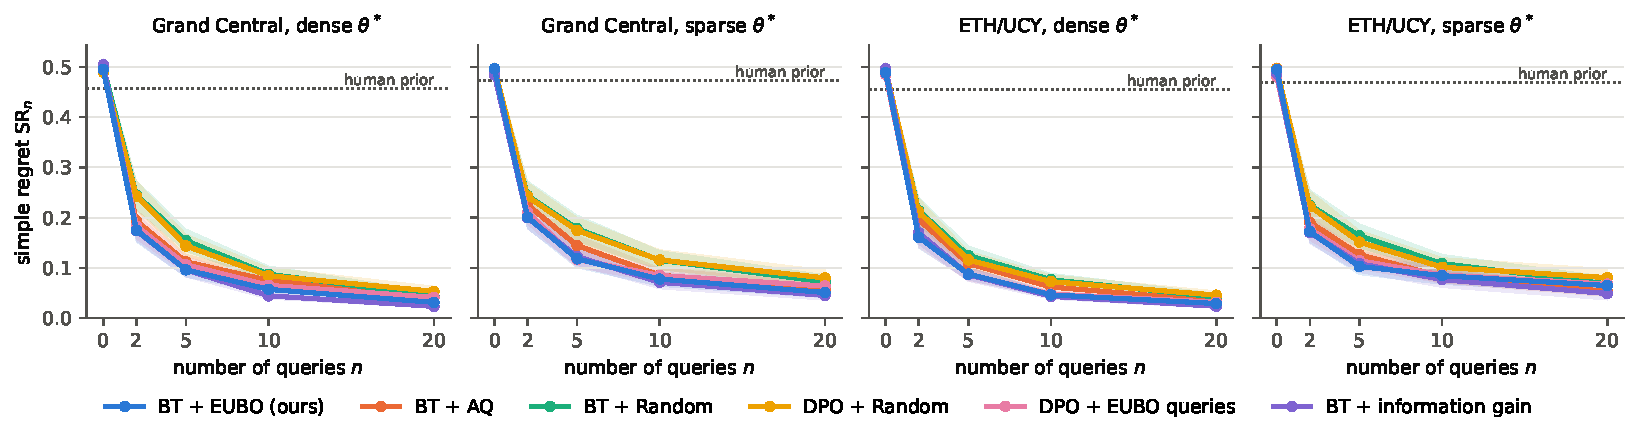
\includegraphics[width=\linewidth]{figures/fig_regret.pdf}
  \caption{Simple regret $\mathrm{SR}_n$ (Eq.~\ref{eq:sr}) on held-out situations against the number of
  A/B queries. Shaded: 95\% bootstrap CI over 200 synthetic users. Dotted: human prior only; the oracle is 0. BT: Bradley--Terry (Laplace); DPO: Sec.~\ref{sec:dpo}.}
  \label{fig:regret}
\end{figure}


\section{Experiments}
\label{sec:experiments}

We ask: (Q1) how quickly does each query method identify a user's style preference on situations the user was never asked about?
(Q2) does the estimator matter, compared with DPO? (Q3) does the candidate generator matter? (Q4) does following the learned preference
in closed loop cost reach or safety?

\subsection{Setup}
\paragraph{Data.} Grand Central~\citep{zhou2012understanding} (GC) and ETH/UCY~\citep{pellegrini2009you,lerner2007crowds}, split by person.
Test situations are held-out pedestrians with a predicted conflict (someone passes within 1\,m in the next 8\,s at constant velocity)
and at least four safe candidates: 12{,}159 on GC (destination $\ge$12\,s ahead) and 590 on ETH/UCY ($\ge$8\,s; Appendix~\ref{app:eth_dest}).
\todo{numbers of training people / samples per dataset}

\paragraph{Users.} Real preferences are unknown, so we use synthetic users: $\theta^\ast \sim \mathcal{N}(0,I)$ normalized
(\emph{dense}: every style matters) or Dirichlet(0.3) magnitudes with random signs (\emph{sparse}: one or two styles dominate),
answering with $\beta=5$ (Sec.~\ref{sec:regret}). Per user, 10 query situations and 20 test situations are drawn without overlap;
200 users per setting; 95\% bootstrap CIs over users.

\paragraph{Baselines.} \emph{Random}: uniformly random pairs. \emph{AQ}: a version-space active query that asks the current best
against its strongest challenger. \todo{cite UserAlign} Both use the same Bradley--Terry estimator as EUBO.

\subsection{Q1: Query selection}
Table~\ref{tab:regret} and Fig.~\ref{fig:regret}. The human-data prior alone leaves a simple regret of 0.45--0.47, close to a random
safe candidate (0.49): the most typical path is not what a given user prefers. Five EUBO queries reduce it to 0.09--0.12 and twenty to
0.03--0.07. With five queries EUBO has lower regret than random queries in all four settings ($-$0.037 to $-$0.061) and than AQ in three
of four ($-$0.021 to $-$0.026; GC dense $-$0.016, n.s.). The gap closes with more queries (20 queries: Table~\ref{tab:regret}, parentheses).
Pairwise agreement shows the same ordering (Appendix, Table~\ref{tab:agreement}).

% Generated by utils/make_paper_tables.py from results/codebook/dpo/{gc,eth}_{gauss,sparse}.json
\begin{table}[t]
\centering
\caption{Simple regret $\mathrm{SR}_n$ (Eq.~\ref{eq:sr}, lower is better) on held-out situations after 5 queries (20 in parentheses). Synthetic users (200 per setting); paired differences after 5 queries with 95\% bootstrap CI over users; $^\dagger$: CI excludes 0. BT: Bayesian Bradley--Terry (Laplace).}
\label{tab:regret}
\setlength{\tabcolsep}{3pt}
\resizebox{\linewidth}{!}{%
\begin{tabular}{lcccc}
\toprule
 & \multicolumn{2}{c}{Grand Central} & \multicolumn{2}{c}{ETH/UCY} \\
\cmidrule(lr){2-3}\cmidrule(lr){4-5}
Method & dense $\theta^*$ & sparse $\theta^*$ & dense $\theta^*$ & sparse $\theta^*$ \\
\midrule
Random safe candidate & 0.492 & 0.493 & 0.495 & 0.490 \\
Human prior only & 0.457 & 0.472 & 0.454 & 0.469 \\
\midrule
BT + random queries & 0.154 \scriptsize{(0.044)} & 0.178 \scriptsize{(0.072)} & 0.125 \scriptsize{(0.042)} & 0.164 \scriptsize{(0.068)} \\
BT + active query (AQ) & 0.112 \scriptsize{(0.041)} & 0.144 \scriptsize{(0.059)} & 0.109 \scriptsize{(0.034)} & 0.126 \scriptsize{(0.053)} \\
DPO + random queries & 0.144 \scriptsize{(0.053)} & 0.174 \scriptsize{(0.080)} & 0.116 \scriptsize{(0.046)} & 0.151 \scriptsize{(0.081)} \\
DPO + EUBO queries & 0.106 \scriptsize{(0.041)} & \textbf{0.117} \scriptsize{(0.064)} & \textbf{0.087} \scriptsize{(0.032)} & 0.114 \scriptsize{(0.068)} \\
BT + EUBO (ours) & \textbf{0.096} \scriptsize{(0.031)} & 0.118 \scriptsize{(0.051)} & 0.088 \scriptsize{(0.029)} & \textbf{0.103} \scriptsize{(0.065)} \\
Oracle $\theta^*$ & 0.000 & 0.000 & 0.000 & 0.000 \\
\midrule
EUBO $-$ Random (5 q) & $-$0.058$^\dagger$ \scriptsize{[$-$0.081, $-$0.034]} & $-$0.060$^\dagger$ \scriptsize{[$-$0.084, $-$0.036]} & $-$0.037$^\dagger$ \scriptsize{[$-$0.059, $-$0.016]} & $-$0.061$^\dagger$ \scriptsize{[$-$0.083, $-$0.039]} \\
EUBO $-$ AQ (5 q) & $-$0.016 \scriptsize{[$-$0.034, +0.001]} & $-$0.026$^\dagger$ \scriptsize{[$-$0.044, $-$0.010]} & $-$0.021$^\dagger$ \scriptsize{[$-$0.037, $-$0.006]} & $-$0.024$^\dagger$ \scriptsize{[$-$0.038, $-$0.009]} \\
EUBO $-$ DPO (5 q) & $-$0.048$^\dagger$ \scriptsize{[$-$0.069, $-$0.026]} & $-$0.056$^\dagger$ \scriptsize{[$-$0.079, $-$0.034]} & $-$0.028$^\dagger$ \scriptsize{[$-$0.049, $-$0.009]} & $-$0.049$^\dagger$ \scriptsize{[$-$0.070, $-$0.027]} \\
\bottomrule
\end{tabular}
}
\end{table}


\subsection{Q2: Estimator -- DPO}
\label{sec:dpo}
DPO~\citep{rafailov2023direct} fits a policy $\pi_\theta(k \mid s) \propto \exp(\theta^\top\phi(s,k))$ to the answered pairs with the
human prior as the reference policy. Because the \emph{human} feature is the standardized log-prior, the reference lies in the same family
($\theta_{\text{ref}} = \sigma_{\text{human}} e_{\text{human}}$) and the DPO loss becomes
$-\log\sigma\bigl(\beta_{\text{DPO}}(\theta - \theta_{\text{ref}})^\top(\phi_w - \phi_l)\bigr)$: a Bradley--Terry likelihood anchored at the
prior, without a posterior. We minimize it by 1{,}000 steps of gradient descent from $\theta_{\text{ref}}$ with $\beta_{\text{DPO}}=0.3$,
the best of ten $(\beta_{\text{DPO}}, \text{steps})$ settings on GC dense (tuned on the evaluation setting, which favours DPO).
Without a posterior DPO cannot choose its questions, so it uses random pairs; \emph{DPO + EUBO queries} receives the pairs EUBO picks.

With the same random questions, DPO and Bradley--Terry are close after five queries and DPO is slightly worse after twenty
(agreement $-$0.005 to $-$0.016). EUBO has lower regret than DPO in all settings ($-$0.028 to $-$0.056 at five queries).
Given EUBO's questions, DPO comes within 0.011 of EUBO: most of the gain comes from choosing the questions, not from the estimator.

\subsection{Q3: Candidate generator}
Table~\ref{tab:generator}. We compare the codebook with the candidates of a flow-matching crowd-navigation planner
\todo{name + cite Crowd-FM; 20 samples refined by PRIEST \todo{cite}} on the 900 GC scenes for which those candidates exist
(150 people $\times$ 6 frames; 811 where both generators have $\ge$4 safe candidates). To make the comparison fair, both are evaluated on
the planner's 3\,s horizon with the people it was given, the same safety filter, and the four features that both can compute
(\emph{human} needs the codebook prior). Because regret normalized within each generator's own set rewards narrow sets, we report
\emph{union regret}, normalized over both generators' safe candidates.

Codebook candidates span a wider range of behaviours (median lateral spread at 3\,s: 2.55\,m vs 0.50\,m). Even an oracle that knows
$\theta^\ast$ cannot get the flow-matching candidates below 0.29--0.32 union regret, against 0.06--0.07 for the codebook. With five EUBO
queries the codebook reaches 0.11 (dense) / 0.15 (sparse) against 0.35 / 0.35. The query-method effect is similar for both generators
(EUBO $-$ random: $-$0.03 to $-$0.05). Restricting to users who dislike detours ($\theta_{\text{detour}}<0$), which removes the users
who favour wide candidate sets by construction, narrows the gap (0.13 vs 0.20 dense) but does not close it.

% Generated by utils/make_paper_tables.py from results/codebook/generator/gc_{gauss,sparse}.json
\begin{table}[t]
\centering
\caption{Candidate generator $\times$ query method on the same 811 Grand Central scenes (first 3\,s, four style features without \emph{human}). Union regret: Eq.~\ref{eq:regret} normalized over the safe candidates of both generators (comparable across generators); own regret: within the generator's own candidates (not comparable). 5 queries (20 in parentheses), 200 synthetic users.}
\label{tab:generator}
\setlength{\tabcolsep}{3pt}
\resizebox{\linewidth}{!}{%
\begin{tabular}{lcccc}
\toprule
 & \multicolumn{2}{c}{dense $\theta^*$} & \multicolumn{2}{c}{sparse $\theta^*$} \\
\cmidrule(lr){2-3}\cmidrule(lr){4-5}
Candidates + queries & union regret & own regret & union regret & own regret \\
\midrule
Crowd-FM + random queries & 0.397 \scriptsize{(0.351)} & 0.225 & 0.384 \scriptsize{(0.344)} & 0.256 \\
Crowd-FM + AQ & 0.368 \scriptsize{(0.336)} & 0.148 & 0.354 \scriptsize{(0.316)} & 0.190 \\
Crowd-FM + EUBO & 0.354 \scriptsize{(0.330)} & 0.111 & 0.351 \scriptsize{(0.318)} & 0.179 \\
Crowd-FM oracle $\theta^*$ & 0.317 & 0 & 0.287 & 0 \\
\midrule
VQ-VAE + random queries & 0.157 \scriptsize{(0.085)} & 0.116 & 0.205 \scriptsize{(0.127)} & 0.163 \\
VQ-VAE + AQ & 0.123 \scriptsize{(0.077)} & 0.078 & 0.162 \scriptsize{(0.101)} & 0.115 \\
VQ-VAE + EUBO (ours) & 0.113 \scriptsize{(0.076)} & 0.066 & 0.154 \scriptsize{(0.108)} & 0.106 \\
VQ-VAE oracle $\theta^*$ & 0.057 & 0 & 0.068 & 0 \\
\midrule
VQ-VAE+EUBO $-$ Crowd-FM+EUBO (5 q) & $-$0.241$^\dagger$ \scriptsize{[$-$0.286, $-$0.202]} &  & $-$0.197$^\dagger$ \scriptsize{[$-$0.241, $-$0.156]} &  \\
Crowd-FM: EUBO $-$ random (5 q) & $-$0.043$^\dagger$ \scriptsize{[$-$0.055, $-$0.033]} &  & $-$0.032$^\dagger$ \scriptsize{[$-$0.045, $-$0.020]} &  \\
VQ-VAE: EUBO $-$ random (5 q) & $-$0.044$^\dagger$ \scriptsize{[$-$0.063, $-$0.026]} &  & $-$0.051$^\dagger$ \scriptsize{[$-$0.073, $-$0.029]} &  \\
\bottomrule
\end{tabular}}
\end{table}


\subsection{Q4: Closed-loop replay}
Table~\ref{tab:closed_loop}. A held-out pedestrian is replaced by the robot, which re-plans every 0.8\,s from the codebook, executes
the first step and must reach the pedestrian's final position; everyone else is replayed and does not react. When no candidate is safe
at cruise speed the robot tries the same paths at half speed and then standing still; the straight final approach is checked the same way.
Following the preference learned from five queries reduces the step regret from about 0.5 to 0.10--0.14 without a significant change in
collision rate; reach drops by 1.7--4.4 points (significant in two of four settings).
Robot-caused collisions remain above the recorded pedestrian's on GC (0.41--0.45 vs 0.21) for every policy including the oracle;
on ETH/UCY the safety-checked approach brings them close for the prior and five-query policies (0.25--0.28 vs 0.24). Most remaining GC collisions occur on steps where a
candidate judged safe under constant-velocity prediction was followed, i.e.\ they come from the prediction model, not from the preference.

% Generated by utils/make_paper_tables.py from results/codebook/closed_loop/{gc,eth}_{gauss,sparse}_safe_c0.5.json
\begin{table}[t]
\centering
\caption{Closed-loop replay (non-reactive pedestrians, re-planning every 0.8\,s, clearance 0.5\,m, collision $<$ 0.4\,m). GC: 300 episodes; ETH/UCY: 114 episodes from 85 people. Robot-caused: the robot's own motion closes the gap faster than the person's at the closest moment. Paired differences with 95\% bootstrap CI.}
\label{tab:closed_loop}
\setlength{\tabcolsep}{3pt}
\resizebox{\linewidth}{!}{%
\begin{tabular}{llcccc}
\toprule
Setting & Policy & reached & collision & robot-caused & step regret \\
\midrule
GC, dense & recorded pedestrian & 1.000 & 0.313 & 0.207 & -- \\
 & human prior & 0.987 & 0.587 & 0.453 & 0.520 \\
 & preference, 5 q & 0.967 & 0.580 & 0.407 & 0.096 \\
 & preference, 20 q & 0.950 & 0.620 & 0.453 & 0.034 \\
 & oracle $\theta^*$ & 0.963 & 0.610 & 0.437 & 0.000 \\
 & 5 q $-$ prior & $-$0.020$^\dagger$ \scriptsize{[$-$0.040, $-$0.003]} & $-$0.007 \scriptsize{[$-$0.073, +0.057]} & $-$0.047 \scriptsize{[$-$0.113, +0.023]} & $-$0.424$^\dagger$ \scriptsize{[$-$0.460, $-$0.387]} \\
\midrule
GC, sparse & human prior & 0.987 & 0.587 & 0.453 & 0.478 \\
 & preference, 5 q & 0.970 & 0.603 & 0.453 & 0.111 \\
 & preference, 20 q & 0.960 & 0.623 & 0.447 & 0.071 \\
 & oracle $\theta^*$ & 0.973 & 0.617 & 0.423 & 0.000 \\
 & 5 q $-$ prior & $-$0.017 \scriptsize{[$-$0.037, +0.000]} & +0.017 \scriptsize{[$-$0.050, +0.080]} & +0.000 \scriptsize{[$-$0.067, +0.067]} & $-$0.367$^\dagger$ \scriptsize{[$-$0.404, $-$0.329]} \\
\midrule
ETH/UCY, dense & recorded pedestrian & 1.000 & 0.325 & 0.237 & -- \\
 & human prior & 1.000 & 0.491 & 0.263 & 0.502 \\
 & preference, 5 q & 0.974 & 0.465 & 0.246 & 0.116 \\
 & preference, 20 q & 0.965 & 0.509 & 0.316 & 0.047 \\
 & oracle $\theta^*$ & 0.965 & 0.491 & 0.351 & 0.000 \\
 & 5 q $-$ prior & $-$0.026 \scriptsize{[$-$0.060, +0.000]} & $-$0.026 \scriptsize{[$-$0.132, +0.079]} & $-$0.018 \scriptsize{[$-$0.108, +0.071]} & $-$0.386$^\dagger$ \scriptsize{[$-$0.445, $-$0.325]} \\
\midrule
ETH/UCY, sparse & human prior & 1.000 & 0.491 & 0.263 & 0.486 \\
 & preference, 5 q & 0.956 & 0.447 & 0.281 & 0.135 \\
 & preference, 20 q & 0.974 & 0.474 & 0.281 & 0.055 \\
 & oracle $\theta^*$ & 0.974 & 0.465 & 0.307 & 0.000 \\
 & 5 q $-$ prior & $-$0.044$^\dagger$ \scriptsize{[$-$0.089, $-$0.009]} & $-$0.044 \scriptsize{[$-$0.148, +0.061]} & +0.018 \scriptsize{[$-$0.073, +0.114]} & $-$0.351$^\dagger$ \scriptsize{[$-$0.426, $-$0.282]} \\
\bottomrule
\end{tabular}}
\end{table}


\subsection{Pilot with real participants}
\todo{If responses are collected before submission: pilot v3 (20 questions; 10 train shown first, 8 test, 2 repeated with sides swapped);
report held-out answer accuracy of the personal $\theta$ vs a shared $\theta$ and the human prior (utils/analyze_pilot.py).
Otherwise move to Limitations. Do not claim IRB exemption unless confirmed.}

\section{Limitations}
\label{sec:limitations}

\paragraph{Synthetic users.} All quantitative results use synthetic users whose answers follow the same Bradley--Terry model the
estimator assumes, which favours model-based estimators; whether real people's walking-style preferences are linear in these features,
stable, and different from each other is for a user study to show. The pilot of Sec.~\ref{sec:pilot} is in progress and reports no
results here; by our power simulation it needs about 20 participants to separate personal from shared preferences when people differ
moderately, and no feasible number suffices if people are nearly alike.

\paragraph{Linear features.} The five features are hand-designed and evaluated at one conflict person; group-related preferences
(cutting through a queue or a conversation) need further features.

\paragraph{Closed loop.} Pedestrians are replayed and do not react to the robot; perception is perfect; the robot is a point with no
dynamics. Robot-caused collisions on GC stay above the recorded pedestrian's for every policy, including the oracle, because the safety
filter relies on constant-velocity prediction. A learned or uncertainty-aware predictor and reactive pedestrians are future work.

\paragraph{Generator comparison.} The flow-matching candidates were available on 900 GC scenes only (3\,s horizon, people in the planner's
window), so the comparison uses that horizon, those people and four features.

\section{Conclusion}
\label{sec:conclusion}
We separated what a crowd-navigation robot can do -- safe paths decoded from a codebook of human walking behaviours -- from which of them a
particular user wants, and learned the latter from a handful of A/B questions. Five EUBO queries cut the simple regret on unseen situations
from that of the human-data prior (0.45--0.47) to 0.09--0.12. The questions matter more than the estimator, and the candidate set bounds
what any preference can achieve. \todo{one sentence on the user study / next steps}


\bibliographystyle{plainnat}
\bibliography{refs}

\appendix
\section{Additional results}

\subsection{Pairwise agreement}
% Generated by utils/make_paper_tables.py from results/codebook/dpo/{gc,eth}_{gauss,sparse}.json
\begin{table}[h]
\centering
\caption{Held-out pairwise agreement with the user's preference (higher is better) after 5 queries (20 in parentheses); same runs as Table~\ref{tab:regret}.}
\label{tab:agreement}
\setlength{\tabcolsep}{3pt}
\resizebox{\linewidth}{!}{%
\begin{tabular}{lcccc}
\toprule
 & \multicolumn{2}{c}{Grand Central} & \multicolumn{2}{c}{ETH/UCY} \\
\cmidrule(lr){2-3}\cmidrule(lr){4-5}
Method & dense $\theta^*$ & sparse $\theta^*$ & dense $\theta^*$ & sparse $\theta^*$ \\
\midrule
Random safe candidate & 0.500 & 0.500 & 0.500 & 0.500 \\
Human prior only & 0.535 & 0.522 & 0.536 & 0.527 \\
\midrule
BT + random queries & 0.789 \scriptsize{(0.902)} & 0.760 \scriptsize{(0.874)} & 0.816 \scriptsize{(0.903)} & 0.780 \scriptsize{(0.872)} \\
BT + active query (AQ) & 0.816 \scriptsize{(0.898)} & 0.793 \scriptsize{(0.876)} & 0.824 \scriptsize{(0.908)} & 0.801 \scriptsize{(0.885)} \\
DPO + random queries & 0.791 \scriptsize{(0.888)} & 0.764 \scriptsize{(0.858)} & 0.820 \scriptsize{(0.897)} & 0.790 \scriptsize{(0.864)} \\
DPO + EUBO queries & 0.822 \scriptsize{(0.897)} & 0.806 \scriptsize{(0.875)} & 0.840 \scriptsize{(0.912)} & 0.817 \scriptsize{(0.876)} \\
BT + EUBO (ours) & \textbf{0.828} \scriptsize{(0.911)} & \textbf{0.809} \scriptsize{(0.892)} & \textbf{0.842} \scriptsize{(0.920)} & \textbf{0.824} \scriptsize{(0.881)} \\
Oracle $\theta^*$ & 1.000 & 1.000 & 1.000 & 1.000 \\
\midrule
EUBO $-$ Random (5 q) & +0.039$^\dagger$ \scriptsize{[+0.021, +0.059]} & +0.049$^\dagger$ \scriptsize{[+0.031, +0.068]} & +0.026$^\dagger$ \scriptsize{[+0.008, +0.047]} & +0.044$^\dagger$ \scriptsize{[+0.025, +0.062]} \\
EUBO $-$ AQ (5 q) & +0.012 \scriptsize{[$-$0.003, +0.027]} & +0.016$^\dagger$ \scriptsize{[+0.001, +0.032]} & +0.019$^\dagger$ \scriptsize{[+0.003, +0.033]} & +0.023$^\dagger$ \scriptsize{[+0.009, +0.039]} \\
EUBO $-$ DPO (5 q) & +0.037$^\dagger$ \scriptsize{[+0.019, +0.056]} & +0.045$^\dagger$ \scriptsize{[+0.028, +0.064]} & +0.022$^\dagger$ \scriptsize{[+0.005, +0.040]} & +0.034$^\dagger$ \scriptsize{[+0.017, +0.052]} \\
\bottomrule
\end{tabular}
}
\end{table}


\subsection{Users outside the estimator's model}
% Generated by utils/make_paper_tables.py from results/codebook/robust/{gc,eth}_*.json
\begin{table}[h]
\centering
\caption{Simple regret after 5 queries for users the estimator does not describe (dense $\theta^*$, 200 users each; the main experiments use $\beta=5$ and linear utilities). $\beta$: answer noise (lower is noisier); random answers: each answer is a coin flip with probability 0.2; nonlinear: pairwise feature interactions with weight $w$ added to the true utility, so the oracle $\theta^*$ no longer reaches 0. $^\dagger$: EUBO's 95\% CI over users is below Random, AQ and DPO.}
\label{tab:robust}
\setlength{\tabcolsep}{3pt}
\resizebox{\linewidth}{!}{%
\begin{tabular}{lccccccc}
\toprule
Users & Prior & Random & AQ & DPO & InfoGain & EUBO & Oracle $\theta^*$ \\
\midrule
\multicolumn{8}{l}{\emph{Grand Central}} \\
answer noise $\beta=1$ & 0.457 & 0.336 & 0.232 & 0.325 & \textbf{0.176} & 0.182$^\dagger$ & 0.000 \\
answer noise $\beta=2$ & 0.457 & 0.241 & 0.155 & 0.232 & \textbf{0.120} & 0.128$^\dagger$ & 0.000 \\
answer noise $\beta=10$ & 0.457 & 0.130 & 0.101 & 0.122 & 0.091 & \textbf{0.085$^\dagger$} & 0.000 \\
20\% random answers & 0.457 & 0.237 & 0.196 & 0.234 & 0.141 & \textbf{0.137$^\dagger$} & 0.000 \\
nonlinear utility, $w=0.5$ & 0.456 & 0.238 & 0.207 & 0.227 & \textbf{0.173} & 0.180$^\dagger$ & 0.090 \\
nonlinear utility, $w=1$ & 0.464 & 0.342 & 0.332 & 0.334 & \textbf{0.301} & 0.303$^\dagger$ & 0.207 \\
\midrule
\multicolumn{8}{l}{\emph{ETH/UCY}} \\
answer noise $\beta=1$ & 0.454 & 0.317 & 0.273 & 0.299 & \textbf{0.174} & 0.206$^\dagger$ & 0.000 \\
answer noise $\beta=2$ & 0.454 & 0.207 & 0.161 & 0.192 & \textbf{0.104} & 0.121$^\dagger$ & 0.000 \\
answer noise $\beta=10$ & 0.454 & 0.098 & 0.094 & 0.095 & \textbf{0.080} & 0.085 & 0.000 \\
20\% random answers & 0.454 & 0.205 & 0.218 & 0.189 & \textbf{0.124} & 0.148$^\dagger$ & 0.000 \\
nonlinear utility, $w=0.5$ & 0.460 & 0.242 & 0.217 & 0.239 & 0.191 & \textbf{0.184$^\dagger$} & 0.095 \\
nonlinear utility, $w=1$ & 0.471 & 0.348 & 0.347 & 0.346 & 0.328 & \textbf{0.317$^\dagger$} & 0.218 \\
\bottomrule
\end{tabular}
}
\end{table}


\subsection{ETH/UCY destination horizon}
\label{app:eth_dest}
% Appendix: ETH/UCY with destination >= 12 s (as GC) vs >= 8 s (main text).
% Sources: results/codebook/style/eth_{gauss,sparse}.json (12 s), results/codebook/dest8/eth_{gauss,sparse}.json (8 s)
\begin{table}[h]
\centering
\caption{ETH/UCY with the destination at least 12\,s ahead (the Grand Central setting; 48 test pedestrians have such a destination, and the 281 evaluation situations come from 41 of them) and at least 8\,s ahead (main text; 88 test pedestrians, 590 situations from 78 of them). Held-out pairwise agreement after 5 queries (20 in parentheses); paired differences after 5 queries with 95\% bootstrap CI over 200 synthetic users.}
\label{tab:eth_dest}
\setlength{\tabcolsep}{4pt}
\begin{tabular}{lcccc}
\toprule
 & \multicolumn{2}{c}{dense $\theta^*$} & \multicolumn{2}{c}{sparse $\theta^*$} \\
\cmidrule(lr){2-3}\cmidrule(lr){4-5}
Method & $\geq$12\,s & $\geq$8\,s & $\geq$12\,s & $\geq$8\,s \\
\midrule
Human prior only  & 0.532 & 0.536 & 0.529 & 0.527 \\
Random queries    & 0.800 \scriptsize{(0.902)} & 0.816 \scriptsize{(0.903)} & 0.786 \scriptsize{(0.877)} & 0.780 \scriptsize{(0.872)} \\
Active query (AQ) & 0.822 \scriptsize{(0.911)} & 0.824 \scriptsize{(0.908)} & 0.789 \scriptsize{(0.874)} & 0.801 \scriptsize{(0.885)} \\
EUBO (ours)       & \textbf{0.850} \scriptsize{(0.915)} & \textbf{0.842} \scriptsize{(0.920)} & \textbf{0.822} \scriptsize{(0.886)} & \textbf{0.824} \scriptsize{(0.881)} \\
\midrule
EUBO $-$ AQ       & +0.028$^\dagger$ \scriptsize{[.012, .044]} & +0.019$^\dagger$ \scriptsize{[.005, .034]} & +0.033$^\dagger$ \scriptsize{[.017, .050]} & +0.023$^\dagger$ \scriptsize{[.008, .038]} \\
EUBO $-$ Random   & +0.050$^\dagger$ \scriptsize{[.031, .069]} & +0.026$^\dagger$ \scriptsize{[.007, .046]} & +0.036$^\dagger$ \scriptsize{[.016, .055]} & +0.044$^\dagger$ \scriptsize{[.027, .063]} \\
\bottomrule
\end{tabular}
\\[2pt]{\scriptsize $^\dagger$ 95\% CI of the paired difference excludes 0.}
\end{table}



\end{document}
